% !TEX root = omar-thesis-proposal.tex
\vspace{-25pt}
\section{Motivation}\label{motivation}
Specifying and implementing a programming language together with its supporting tools (collectively, a \emph{programming system}) that has sound theoretical foundations, helps users identify and fix errors as early as possible, supports a natural programming style, and performs well across diverse problem domains and hardware platforms remains a grand challenge in computing. Due to the increasing diversity and complexity of modern problem domains and hardware platforms, it has become clear that no small  collection of general-purpose constructs backed by a simple, all-purpose implementation can fully satisfy these criteria in all cases. Instead,  researchers and domain experts (collectively, \emph{providers}) continue to develop  specialized notations,  type systems, semantics, implementation strategies, optimizations, run-time systems and tools (collectively, \emph{features})  designed to address these modern challenges in different circumstances. %, researchers and domain experts must continue to design and develop, in a principled manner, specialized notations, type systems, optimizations, run-time systems and tools (collectively, \emph{features}) to support developers as they work in increasingly complex problem domains and on modern hardware systems.

% Rather, researchers and domain experts must continue, in a principled manner, to specify and implement novel abstractions, provide alternative implementations of existing abstractions, supplement languages with useful tools and improve tools with new behaviors (collectively, realize new \emph{features}) that better satisfy these criteria by balancing the concerns relevant to particular application domains. 

Ideally, a provider would develop and distribute such new features orthogonally, as libraries, so that client developers could granularly choose those that best satisfy their needs. Unfortunately this is often infeasible because libraries are vehicles for specifying a program in terms of a monolithic collection of existing features. From the perspective of a library, the language's syntax, type system and semantics are fixed in advance, the compiler and run-time system are ``black box'' implementations of this fixed language, and the other tools, like code editors and debuggers, operate according to domain-agnostic protocols also based only on a fixed language specification. As a result, providers of new system features must typically take \emph{language-external approaches}, sometimes designing a new language altogether. We will argue that such approaches are problematic, and that taking them has led to an unnecessary gap between research and practice. In place of these approaches, we will advocate for \emph{language-integrated extensibility mechanisms}, and show how, by organizing new features around {types} and imposing certain constraints, these mechanisms can be made both safe and highly expressive. We call a type that introduces new features an \emph{active type} and programming systems organized around active types \emph{actively-typed programming systems}.
%But taking a \emph{language-internal approach} to implementing a feature is the most practical. If a feature can be realized by creatively using existing language constructs and distributed as a library, clients face fewer barriers to adoption because it is easy to integrate library-based features into existing projects gradually and granularly and they leverage well-understood and well-developed mechanisms.
% But taking this approach is often \emph{not} possible today %We call designs \emph{monolithic programming systems}.

%To realize a new abstraction or system behavior, such experts can consider either a \emph{language-internal approach}, where they work within an existing language and distribute their solutions as libraries, or a \emph{language-external approach}, where they create a new, distinct programming system (often centered around what has come to be called a new \emph{domain-specific language} \cite{dsl}) or extend an existing system by some mechanism that is not part of the language itself, such as an extension mechanism supported by a {particular} compiler, editor or other tool.
\subsection{Motivating Example: Regular Expressions}\label{regex}
To make the issue concrete, let us begin with a simple example. \emph{Regular expressions} are a widely-used mechanism for finding patterns in semi-structured strings (e.g. DNA sequences) \cite{Thompson:1968:PTR:363347.363387}. A programming system that included full compile-time and edit-time support for regular expressions might simultaneously provide features like these:

\begin{enumerate}
\item \textbf{Built-in syntax for pattern literals} (e.g. \cite{perlre}) so that malformed patterns result in intelligible \emph{compile-time} parsing errors. In languages lacking such literals, run-time errors relating to pattern syntax can occur, even in well-tested, deployed code \cite{spishak2012type}. 
\item \textbf{Typechecking logic} that ensures that key constraints related to regular expressions are not violated at compile-time:
	\begin{enumerate}
	\item only appropriate values are spliced into regular expressions, to avoid splicing errors and injection attacks \cite{owasp2013}
	\item out-of-bounds backreferences are not used \cite{spishak2012type}
	\item strings known to be in the language of a regular expression are given a type that tracks this information and ensures that string manipulation operations do not inadvertently lead to a string that is not in the assumed language \cite{fulton-thesis}.
	\end{enumerate}
When a type error is found, an intelligible error message is provided.
\item \textbf{Elaboration logic} that partially or fully compiles known regular expressions into the efficient internal representation that will be used by the regular expression matching engine (e.g., a finite automata \cite{Thompson:1968:PTR:363347.363387}) ahead of time. In most languages, this compilation step occurs at run-time, even if the pattern is fully known at compile-time, thereby introducing performance overhead into programs. If the developer is not careful to cache compiled representations, regular expressions used repeatedly in a program might be needlessly re-compiled on each use. %By performing this step ahead-of-time, these dangers can be avoided.
\item \textbf{Editor services} for quickly testing regular expression patterns against test strings,  referring to documentation or searching databases of common patterns (e.g. \cite{IntelliJRegexp}).
\end{enumerate}

%In a conventional \emph{monolithic} programming system, support for each of these features would need to be built into the language and tools. 
No system today has built-in support for all of the features enumerated above. Instead, libraries generally provide support for regular expressions by leveraging  general-purpose constructs. Unfortunately, it is impossible to fully encode the syntax and the specialized static and dynamic semantics described above in terms of general-purpose notations and abstractions. Library providers have thus needed to compromise. The typical choice is to have clients provide regular expressions as strings, deferring parsing, typechecking and elaboration to run-time, which introduces performance overhead and can lead to unanticipated run-time errors (as shown in \cite{spishak2012type}) and security vulnerabilities (due to injection attacks when user inputs are spliced into patterns, for example). Similarly, tools are rarely integrated into editors, and even more rarely in a way that facilitates their discovery and use directly when the developer is manipulating regular expressions. Tools that must be discovered independently and accessed externally (for example, via a browser) are used less frequently  and can be more awkward than necessary \cite{Campbell:2008:DRT:1636642.1636651, Omar:2012:ACC:2337223.2337324}, leading to lower productivity.

\subsection{Language-External Approaches}
\begin{figure}
\begin{center}
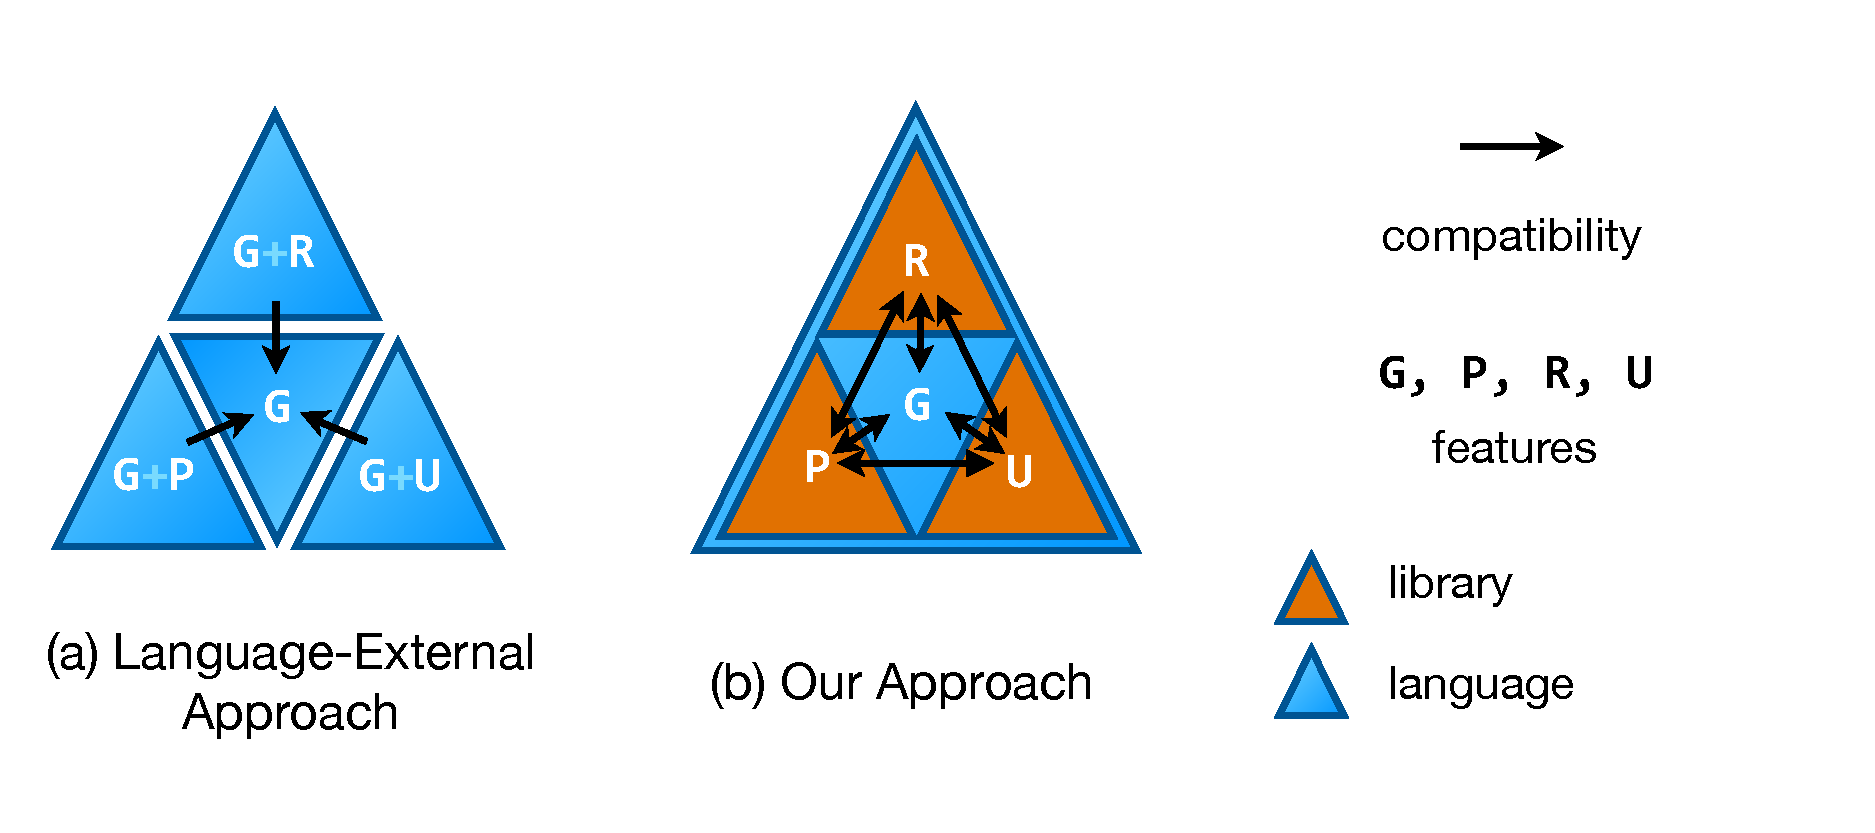
\includegraphics[scale=0.45]{approaches.pdf}
\end{center}
\vspace{-20px}
\caption{\small (a) With the language-external approach, novel features are packaged into separate languages and tools. Clients of an API can only safely and naturally use it if the interface uses common constructs (the \emph{compatibility problem}). (b) With the active library approach, there is one extensible host language and the compile-time and edit-time logic governing novel constructs is expressed within libraries. If the extension mechanism guarantees the safety of arbitrary compositions of extensions, the necessary primitives can simply be imported by library clients as needed, and so interoperability is not a problem.}
\label{approaches}
\end{figure}

When the primitive behaviors of a system must be extended to fully realize a new feature, as in the example above, providers typically take a \emph{language-external approach}, either by developing a new or derivative programming system (often centered around a so-called \emph{domain-specific language (DSL)} \cite{fowler2010domain}) or by extending an existing system by some mechanism that is not part of the language itself, such as an extension mechanism for a {particular} compiler\footnote{Compilers that modify, or allow modification of, the semantics of their base language, rather than simply permitting meaning-preserving optimizations, should be considered a pernicious means for creating new languages. Many ``practical'' compilers, including \texttt{gcc}, \texttt{GHC} and \texttt{SML/NJ}, are guilty of this sin, meaning that some programs that seem to be written in C, Haskell or Standard ML are actually written in tool-specific derivatives of those languages. Language-internal mechanisms do not lead to such fragmentation.} or other tool\todo{relate to regex example and update figure}. %This latter method couples the semantics of the feature to the implementation details of a particular tool. Because the use of one implementation entails a different semantics for the feature than another, the extended tool acts, \emph{de facto}, as a distinct system for our purposes. 

Unfortunately, when providers of new features take language-external approaches, it causes problems for clients that hinder adoption. Features cannot be adopted individually, but instead are only available coupled to a collection of other unrelated  features (e.g. the incidental features of a newly-designed language or tool, or of the particular tool that was extended). This makes adoption more costly when these incidental features are  not appropriate or insufficiently developed, or when the features bundled with a different language or tool are simultaneously desirable. For example, although evidence suggests that developers prefer language-integrated parallel programming abstractions to library-based implementations if all else is equal \cite{langvslib}, library-based implementations are more widely adopted because ``parallel programming languages'' provide full support only for a few chosen parallel programming abstractions along with a small collection of less-developed general-purpose abstractions. This is problematic because different parallel abstractions are more appropriate in different situations \cite{ecoopstudy13} and parallel programming support is rarely the only concern relevant to client developers outside of a classroom setting. Regular expression support, for example, may be simultaneously desirable when processing large amounts of textual data in parallel. %Similarly, a language and tools designed primarily to support regular expressions might make an interesting research project, but it would not be a suitable tool for writing large applications with more varied needs.

%\item Developing a new language and its associated tools places a significant development burden on providers who may wish only to promote a few core innovations, although tools like compiler generators, language workbenches and easy-to-extend tools can decrease this burden. 
%\item 

%Clients seem to prioritize the ability to choose different features for different portions of an application. 
%If calling between languages were safe and easy, then using a variety of specialized languages and associated tools might be less problematic. In fact, s
%Recognizing the limitations of relying on monolithic collection of primitives, some researchers have advocated instead for a model where multiple languages used within a single application, calling it the \emph{language-oriented approach} to software development \cite{languageoriented}. 

Various concerns can sometimes be separated into different components, each written using a suitable language and tooling. This has been called the \emph{language-oriented approach} to software development \cite{language-oriented} and is supported by \emph{language workbenches} \cite{workbenches} and domain-specific language (DSL) frameworks \cite{fowler10}. Unfortunately, this is insufficient: the interfaces between components written in different languages remains an issue. The specialized constructs particular to one language (e.g. futures in a parallel programming language) cannot always be safely and naturally expressed in terms of those available in another (e.g. a general-purpose language), so building a program out of components written in a variety of different languages is difficult whenever these are exposed at interface boundaries. Tool support is also lost when calling into a different language. We call this fundamental issue the \emph{compatibility problem}. 

One strategy often taken by proponents of the language-oriented approach to partially address the compatibility problem is to  target an established intermediate language, such as the Java Virtual Machine (JVM) bytecode\todo{mention functional IL} and support a superset of its constructs. Scala \cite{scala} and F\# \cite{fsharp} are examples of prominent general-purpose languages that have taken this approach, and most DSL frameworks also rely on this strategy. This only enables full interoperability in one direction (Figure \ref{approaches}a). While calling into the common language becomes straightforward, calls in the other direction, or between the languages sharing the common target, are still restricted by the semantics of the common language. 

If new languages only include constructs that can already be expressed safely and reasonably naturally in the common language, then this approach can work well. 
But many of the most innovative constructs found in modern languages (often, the features that justify their creation) are difficult to define in terms of existing constructs in ways that guarantee all necessary invariants are statically maintained and that do not require large amounts boilerplate code and run-time overhead. For example, the type system of F\# guarantees that null values cannot occur within F\# data structures, but maintaining this important invariant still requires run-time checks because the typing rules of F\# do not apply when F\# code is called from other languages on the Common Language Infrastructure (CLI) like C\#. The F\# type system also includes support for checking that units of measure are used correctly \cite{fsharpunits}, but this specialized invariant is left completely unchecked at language boundaries. 
%In Scala, traits that have default method implementations are difficult to implement from Java or other JVM languages and the workaround can break if the trait is modified \cite{scalatraitinterop}. 
In some cases, desirable features must be omitted entirely due to concerns about  interoperability. F\#, for example, aims to maintain compatibility with ML, but due to the need for bidirectional interoperability with CLI languages, it cannot support modules or functors.
%\end{itemize}

\subsection{Language-Integrated Approaches}
We argue that, due to these compatibility problems, taking a language-external approach to realizing a new feature should be considered harmful and avoided whenever possible. The goal of the research being proposed here is to design \emph{language-integrated extension mechanisms} that give developers control over edit-time and compile-time behaviors that have previously been defined centrally\footnote{One might compare today's monolithic programming systems to  {centrally-planned} economies, whereas extensible\- systems more closely resemble modern market economies.} so that such language-external approaches are less frequently necessary. More specifically, we will show how control over \textbf{parsing}, \textbf{typechecking}, \textbf{elaboration} and \textbf{code completion} can be delegated to user-defined logic distributed in {libraries}, as illustrated in Figure \ref{approaches}b. 
Such libraries are called \emph{active libraries} because, rather than being passive clients of features already available in the system, they contain logic invoked by the system during development or compilation to provide new features  \cite{active-libraries}. Features implemented within active libraries are imported as needed by the clients of libraries that rely on them, unlike features implemented by language-external means, avoiding the compatibility problem.

We must proceed with caution, however: critical issues having to do with {safety} must be overcome before library-based extension mechanisms can be introduced into a programming system, because if too much control over such core aspects of the system is given  to developers, the system may become unreliable. 
%For example, an extension could weaken important metatheoretic guarantees previously provided by the system. 
Type safety, for example, may not hold if the static and dynamic semantics of the language can be modified or extended arbitrarily from within libraries. Furthermore, even if extensions can be shown not to cause such problems in isolation, there may still be conflicts between extensions that could weaken their semantics and lead to subtle problems at link-time. For example, if two active libraries defined differing semantics for the same syntactic form, the issue would only manifest itself when both libraries were imported somewhere within the same program. These kinds of safety issues have plagued previous attempts to design language-integrated extensibility mechanisms.% To prevent them, our mechanisms will organize  extension logic around types to guarantee that extensions are both safe in isolation and also safely composable in any combination. 


 %This represents a minimalist approach to system design -- the conventional distinction between built-in and user-defined constructs is blurred and most features of the system are orthogonally implemented as {libraries}, rather than by the maintainers of the system.

%The mechanisms we describe will do so primarily by delimiting the scope of an extension to expressions of a single user-defined type or family of types. 

%This can be thought of as a more pernicious form of the conflict that arises when two globally-accessible constructs are given the same name. n languages without universal namespacing mechanisms (e.g. C, JavaScript, \LaTeX, ML and many others). 

%The extension mechanism\todo{elaborate on safety requirements + tension between expressiveness and safety, merge with next paragraph}. must be expressive enough to allow users to associate rich run-time, compile-time and edit-time behaviors with user constructs directly, while being sufficiently restrictive to maintain the global safety properties of the language and system as a whole, and to ensure that constructs cannot interfere with one another. 
